\documentclass[border=6pt]{standalone}
\usepackage[T1]{fontenc}
\usepackage{lmodern}
\usepackage{tikz}
\usetikzlibrary{positioning, arrows.meta, decorations.pathreplacing, calc, fit}

\begin{document}
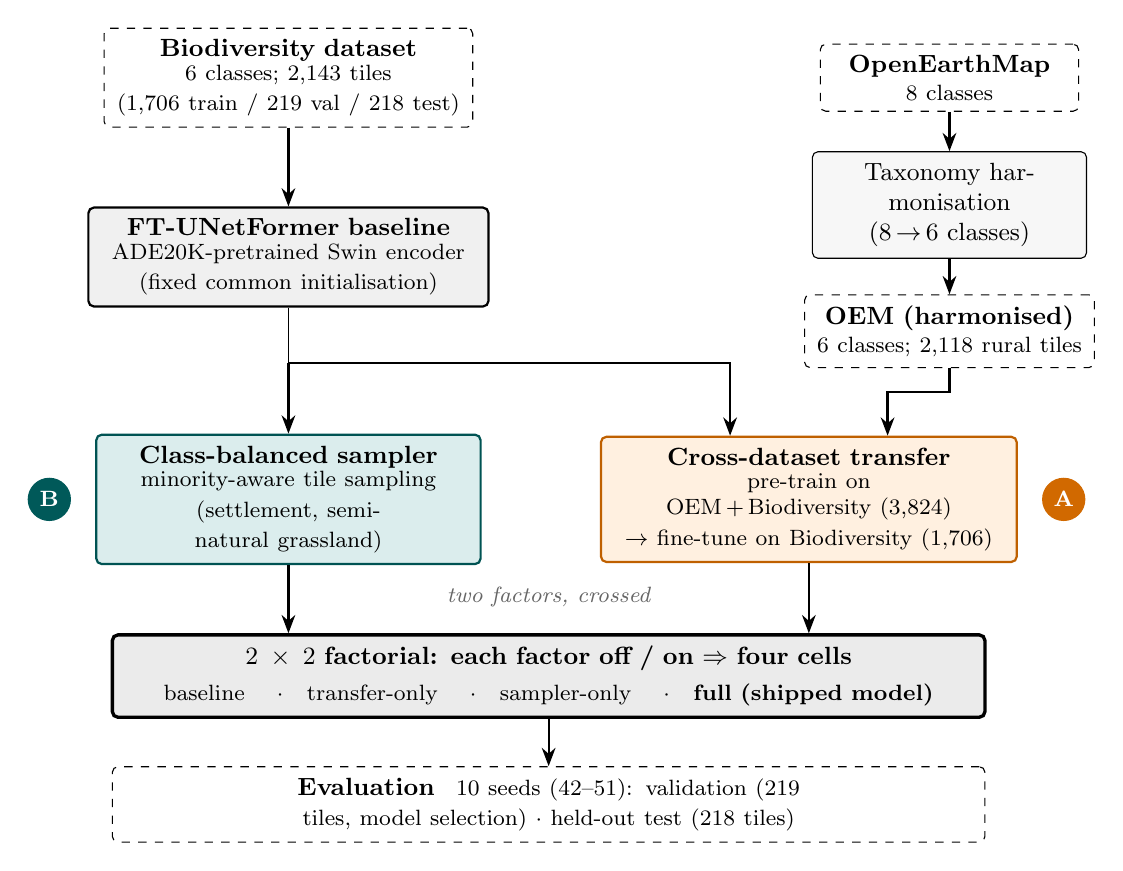
\begin{tikzpicture}[
  font=\small,
  >=Stealth,
  data/.style={draw, dashed, rounded corners=2pt, align=center, inner sep=4pt, fill=white},
  proc/.style={draw, rounded corners=2pt, align=center, inner sep=4pt, fill=gray!6},
  base/.style={proc, thick, fill=gray!12, text width=4.8cm},
  leverA/.style={proc, thick, text width=5.0cm, fill=orange!12, draw=orange!75!black},
  leverB/.style={proc, thick, text width=4.6cm, fill=teal!14, draw=teal!65!black},
  factbox/.style={proc, very thick, fill=gray!16, text width=10.8cm},
  evalb/.style={data, text width=10.8cm},
  badgeA/.style={circle, fill=orange!82!black, text=white, font=\footnotesize\bfseries, inner sep=0pt, minimum size=5.5mm},
  badgeB/.style={circle, fill=teal!70!black, text=white, font=\footnotesize\bfseries, inner sep=0pt, minimum size=5.5mm},
  arr/.style={->, thick},
]

% ---- data sources ----
\node[data, text width=4.4cm] (bio) {\textbf{Biodiversity dataset}\\[-1pt]{\footnotesize 6 classes; 2{,}143 tiles\\(1{,}706 train / 219 val / 218 test)}};
\node[data, right=4.4cm of bio, text width=3.0cm] (oem) {\textbf{OpenEarthMap}\\[-1pt]{\footnotesize 8 classes}};
\node[proc, below=0.5cm of oem, text width=3.2cm] (tax) {Taxonomy harmonisation\\(8\,$\rightarrow$\,6 classes)};
\node[data, below=0.45cm of tax, text width=3.4cm] (oem6) {\textbf{OEM (harmonised)}\\[-1pt]{\footnotesize 6 classes; 2{,}118 rural tiles}};
\draw[arr] (oem) -- (tax);
\draw[arr] (tax) -- (oem6);

% ---- fixed baseline (common initialisation) ----
\node[base, below=1.0cm of bio] (base) {\textbf{FT-UNetFormer baseline}\\[-1pt]{\footnotesize ADE20K-pretrained Swin encoder\\(fixed common initialisation)}};
\draw[arr] (bio) -- (base);

% ---- the two crossed factors ----
\node[leverB, below=1.6cm of base] (lb) {\textbf{Class-balanced sampler}\\[-1pt]{\footnotesize minority-aware tile sampling\\(settlement, semi-natural grassland)}};
\node[badgeB, left=3mm of lb] {B};
\node[leverA, right=1.5cm of lb] (la) {\textbf{Cross-dataset transfer}\\[-1pt]{\footnotesize pre-train on OEM\,+\,Biodiversity (3{,}824)\\$\rightarrow$ fine-tune on Biodiversity (1{,}706)}};
\node[badgeA, right=3mm of la] {A};

% baseline forks into both factors
\coordinate (f) at ($(base.south)+(0,-0.7)$);
\draw (base.south) -- (f);
\draw[arr] (f) -| (lb.north);
\draw[arr] (f) -| ([xshift=-1.0cm]la.north);
% OEM (harmonised) feeds the transfer pre-training (enters the top-right, clear of badge A)
\draw[arr] (oem6.south) -- ++(0,-0.3) -| ([xshift=1.0cm]la.north);

% label the crossing
\node[font=\footnotesize\itshape, text=black!60] at ($(lb.south)!0.5!(la.south)+(0,-0.42)$) {two factors, crossed};

% ---- factorial cells ----
\coordinate (mid) at ($(lb)!0.5!(la)$);
\node[factbox, below=1.7cm of mid] (fact) {\textbf{$2\times2$ factorial: each factor off / on $\Rightarrow$ four cells}\\[2pt]
  {\footnotesize baseline \quad$\cdot$\quad transfer-only \quad$\cdot$\quad sampler-only \quad$\cdot$\quad \textbf{full (shipped model)}}};
\draw[arr] (lb.south) -- (lb.south |- fact.north);
\draw[arr] (la.south) -- (la.south |- fact.north);

% ---- evaluation ----
\node[evalb, below=0.6cm of fact] (eval) {\textbf{Evaluation} \, {\footnotesize 10 seeds (42--51): validation (219 tiles, model selection) $\cdot$ held-out test (218 tiles)}};
\draw[arr] (fact) -- (eval);

\end{tikzpicture}
\end{document}
